\documentclass{article}
    \usepackage{amsmath}
    \usepackage{setspace}
    \usepackage{graphicx} %插入图片的宏包
    \usepackage{float} %设置图片浮动位置的宏包
    \usepackage{subfigure} %插入多图时用子图显示的宏包
   \usepackage{geometry}
    \geometry{a4paper,scale=0.7}
    \usepackage{pythonhighlight}
    \usepackage{longtable}


    %++++++++++++++++++++++++TITLE++++++++++++++++++++++
    \title{The Linear Algebra Apllied in Neural Network}
    \author{CHEN Ming-yu\\2017200506032\\
    \and FENG Cheng-lin\\2017200506035\\
    \and YU Hong-ze\\2017200506034\\}
    \date{June 10 2018}
    
    %++++++++++++++++++++++++SETTING+++++++++++++++++++++
    \begin{document}
    \maketitle
    \begin{spacing}{2}
    \linespread{2}
    %+++++++++++++++++++++++BEGIN REPORT++++++++++++++++
    \section{Abstract}

    \section{Introduction}

    \section{Algorithm}

    Fully connect neural network with proper activate function is a non-linear algorithm which is capable to solve classification problems for the items with multiple features. Unlike a function in traditional concept, a fully connect neural network propagates the input-the features of items waited to be classified-through several layers of neuros and obtain the final outcomes in last layer, and each neuro must represent a non-linear. The propagation, in detail, is to take the output of previous as the input of previous. For one neuro, the independent parameter of the function is the sum of the product of each neuro in previous layer and its corresponding adjustable weight. The advantage of fully connect neural network is the absence of deduction of expression. Once the network was constructed,the structure is optimized by iteration. 

    \section{Mathmatic Expression}

    In terms of the mathematic expression of this algorithm, we discuss a simpler version, two features with on layer of four neuros and an output, compared with the structure we used.\\

    \begin{figure}[H]
        \centering 
        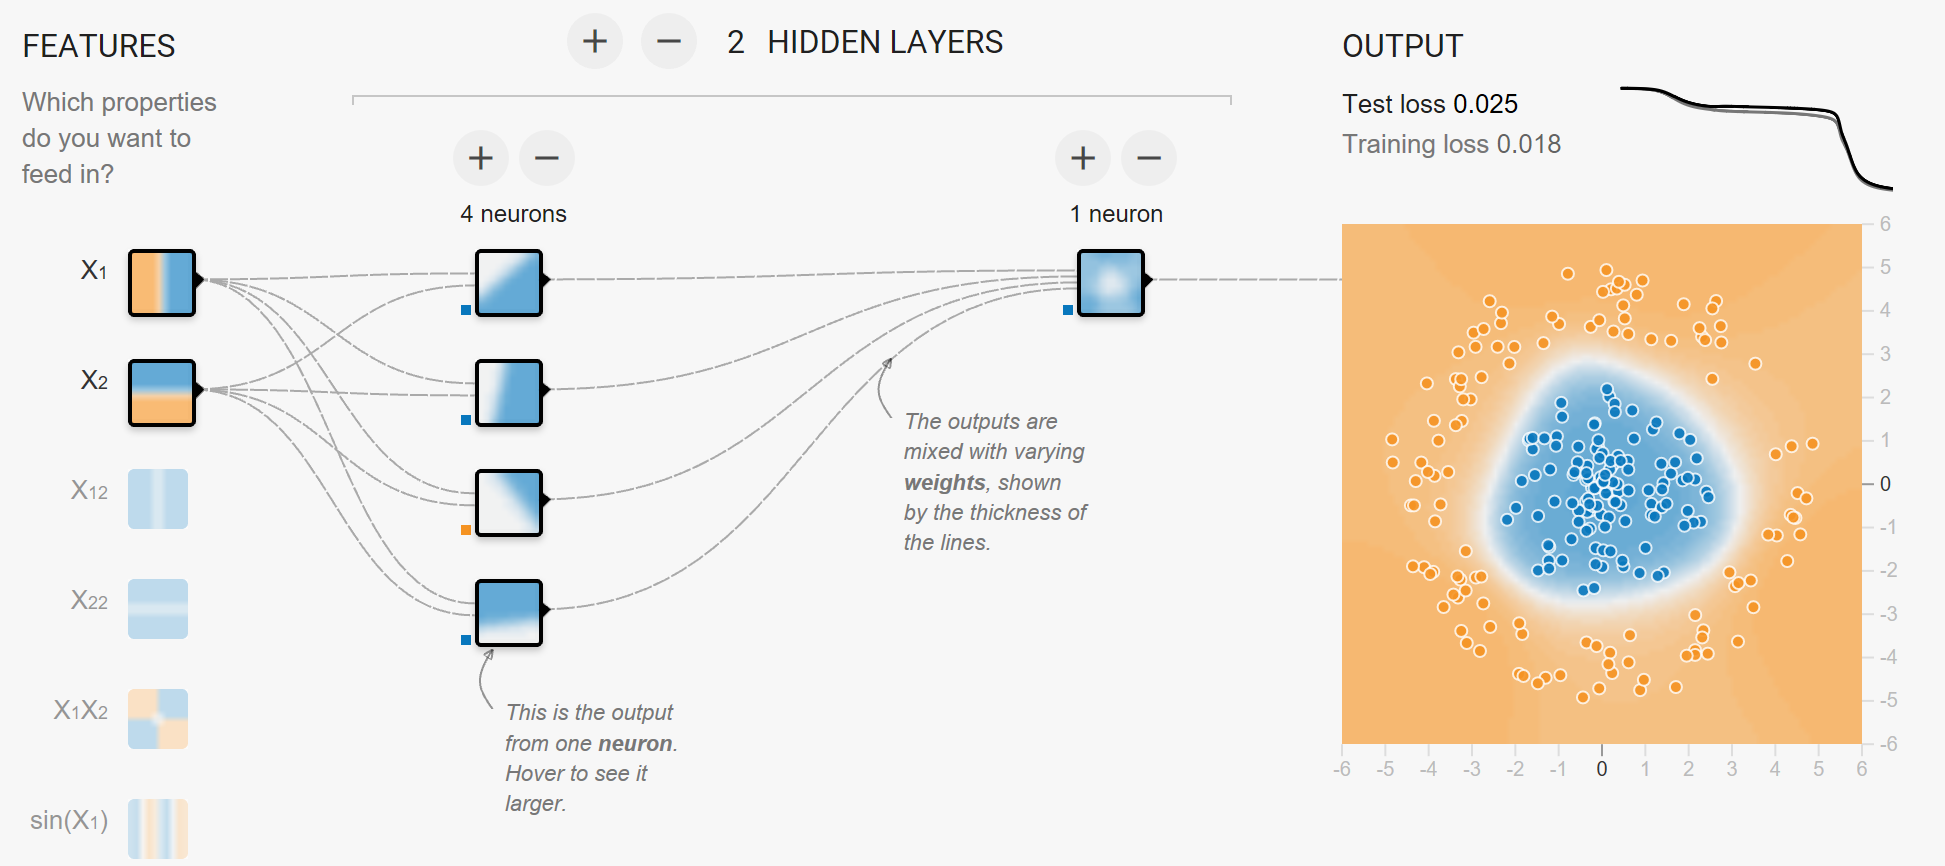
\includegraphics[width=1\textwidth]{TF_Playground}
        \caption{A simplified version\cite{TF_Playground}}
        \end{figure} 
        
    \noindent The sum of the product of outputs and weights is converted into matrix product by introducing the property of inner product in linear algebra. The matirx (\ref{equation1}) represents the features of the each single items that we study, and matrix (\ref{equation2}) represents the weights on the lines connecting the nods in first layger and second, which is showen in figure above.

    \begin{equation}\label{equation1}
        {\left[ \begin{array}{c}
            x_{inputs}
            \end{array}\right]}=
        {\left[ \begin{array}{cc}
        x_1 & x_2
        \end{array}\right]}
    \end{equation}

    \begin{equation}\label{equation2}
        W^{(1)}=
        {\left[ \begin{array}{cccc}
        W^{(1)}_{1,1} & W^{(1)}_{1,2} & W^{(1)}_{1,3} & W^{(1)}_{1,4}\\
        W^{(1)}_{2,1} & W^{(1)}_{2,2} & W^{(1)}_{2,3} & W^{(1)}_{2,4}\\
        \end{array}\right]}
    \end{equation}\\

    \noindent By implementing dot multiple, the value of features propagate to the second layger, the matrix (\ref{equation3}). The same approach are used to calculate final output. (NB: sigmoid funtcion is uesd to cancel linearity.)
        \begin{align}\label{equation3}
        a_{layer}&=
        {\left[ \begin{array}{cccc}
       a_1&a_2&a_3&a_4
        \end{array}\right]}
        =f_{sigmoid}(x_{inputs}W^{(1)})
        =f(
        {\left[ \begin{array}{cc}
            x_1 & x_2
        \end{array}\right]}
        {\left[ \begin{array}{cccc}
            W^{(1)}_{1,1} & W^{(1)}_{1,2} & W^{(1)}_{1,3} & W^{(1)}_{1,4}\\
            W^{(1)}_{2,1} & W_{2,2} & W^{(1)}_{2,3} & W_{2,4}\\
        \end{array}\right]})\nonumber\\
        &=
        {\left[ \begin{array}{ccccc}
            f(W^{(1)}_{1,1}x_1+W^{(1)}_{2,1}x_2) & f(W^{(1)}_{1,2}x_1+W^{(1)}_{2,2}x_2) &f(W^{(1)}_{1,3}x_1+W^{(1)}_{2,3}x_2) &f(W^{(1)}_{1,4}x_1+W^{(1)}_{2,4}x_2)
        \end{array}\right]}
    \end{align}  

    \begin{align*} 
        {\left[ \begin{array}{c}
        y_{output}
        \end{array}\right]}&=
        a_{layer}W^{(2)}
        ={\left[ \begin{array}{cccc}
            a_1&a_2&a_3&a_4
             \end{array}\right]}
        {\left[ \begin{array}{c}
            W^{(2)}_{1,1}\\
            W^{(2)}_{2,1}\\
            W^{(2)}_{3,1}\\
            W^{(2)}_{4,1}\\
        \end{array}\right]}\\
        &={\left[ \begin{array}{c}
            W^{(2)}_{1,1}a_1+W^{(2)}_{2,1}a_2+W^{(2)}_{3,1}a_3+W^{(2)}_{4,1}a_4
        \end{array}\right]}
    \end{align*}

    \noindent However, the initial outcome may not be correct indicating the network needs improvement. The formula we used to reflect the distance between the outcome and the labeled correct answer is the cross entropy, which is capable to reflect the distance between two probability distribution. 

    \begin{center}
    $H(p_{labeled},q_{outcome})=$$\sum_{i}p_i{\times}log_2(\frac{1}{q_i})$\\
    \end{center}

    \noindent The problem we study we studied was converted into binary distribution with labeled wanted item ”1” and unwanted item “0”. Thus, after mapping the results within 0 to 1, the propagation outcome naturally becomes a binary. Then update each laments in weights matrixes by subtracting the gradients of cross entropy (the loss function). According to the figure above, the performance is acceptable after roughly 3000 steps.
    
    \section{Algorithmic Realization}

    To simplified the coding complexity, a python module TesnorFlow\cite{TensorFlow} was introduced. The algorithe was realized in python environment with Jupyter\cite{Jupyter}. We conducted a survey enquiring the 5 different factors,height,weight,chest, waist and hip sizes, to determine wheter a male is charming or not.\\

    \begin{figure}[H]
        \centering 
        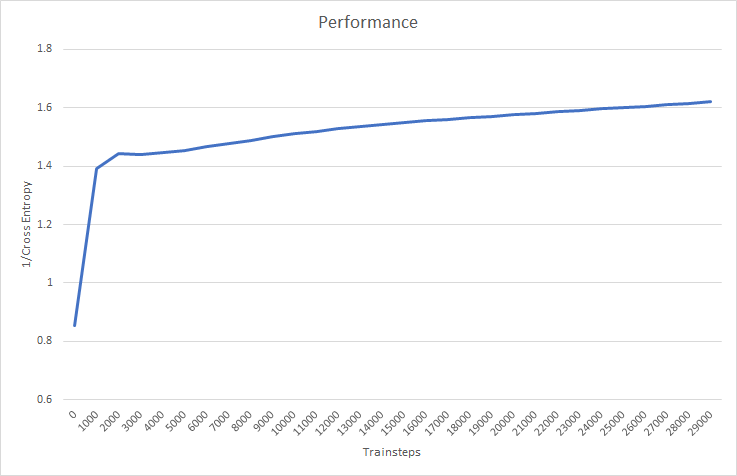
\includegraphics[width=1\textwidth]{Performance}
        \caption{Performance through out 30000 training stpes.\cite{Performance}}
        \end{figure}
  
    \noindent For each train step, the network picks out eight five dimentional teature vector whoes elements are the data for one meal reported form sbujects. Then follow the process mentioned above to implement gradient descend. The reciprocal of cross entropy is used to indicate the perofrmance (or accuracy). 

    

    \section{Conclutsion}


    \section{Appendix}

    \begin{center}
    \textbf{Training Sets}\\
    \setlength{\tabcolsep}{7mm}{
    \begin{longtable}{cccccc} \toprule
    Y$\backslash$N  &  Height  &  Weight  &  Chest  &  Waist &  Hip \\ \hline
1   & 177 & 73  & 96  & 80  & 94 \\
1   & 175 & 71  & 103 & 84  & 97 \\
1   & 182 & 72  & 102 & 81  & 102 \\
1   & 174 & 67  & 102 & 81  & 97 \\
1   & 183 & 69  & 103 & 80  & 94 \\
1   & 167 & 70  & 95  & 88  & 96 \\
1   & 168 & 73  & 101 & 81  & 99 \\
1   & 167 & 70  & 99  & 81  & 98 \\
1   & 176 & 68  & 103 & 83  & 96 \\
1   & 176 & 72  & 97  & 80  & 102 \\
1   & 173 & 70  & 97  & 83  & 99 \\
1   & 173 & 71  & 96  & 84  & 99 \\
1   & 172 & 72  & 100 & 88  & 99 \\
1   & 174 & 71  & 97  & 88  & 100 \\
1   & 172 & 73  & 97  & 88  & 98 \\
1   & 183 & 70  & 97  & 85  & 98 \\
1   & 171 & 70  & 99  & 85  & 98 \\
1   & 177 & 68  & 101 & 84  & 97 \\
1   & 179 & 68  & 95  & 81  & 99 \\
1   & 169 & 73  & 99  & 85  & 102 \\
1   & 179 & 69  & 95  & 86  & 101 \\
1   & 174 & 68  & 97  & 86  & 99 \\
1   & 177 & 68  & 99  & 80  & 99 \\
1   & 178 & 73  & 100 & 84  & 96 \\
1   & 171 & 71  & 102 & 82  & 98 \\
1   & 177 & 72  & 99  & 80  & 100 \\
1   & 170 & 68  & 102 & 88  & 98 \\
1   & 173 & 72  & 96  & 83  & 97 \\
1   & 168 & 71  & 95  & 81  & 94 \\
1   & 169 & 69  & 97  & 86  & 98 \\
1   & 181 & 69  & 100 & 86  & 100 \\
1   & 172 & 70  & 96  & 83  & 98 \\
1   & 177 & 68  & 102 & 81  & 100 \\
1   & 169 & 67  & 97  & 85  & 95 \\
1   & 175 & 67  & 95  & 82  & 102 \\
1   & 169 & 67  & 98  & 83  & 101 \\
1   & 177 & 69  & 97  & 82  & 96 \\
1   & 174 & 73  & 100 & 81  & 97 \\
1   & 177 & 69  & 103 & 82  & 96 \\
1   & 171 & 72  & 95  & 82  & 97 \\
1   & 181 & 68  & 99  & 81  & 97 \\
1   & 173 & 71  & 99  & 84  & 99 \\
1   & 181 & 70  & 97  & 80  & 97 \\
1   & 168 & 70  & 98  & 81  & 99 \\
1   & 177 & 71  & 98  & 85  & 97 \\
1   & 173 & 68  & 97  & 86  & 97 \\
1   & 175 & 67  & 102 & 86  & 99 \\
1   & 180 & 68  & 100 & 81  & 95 \\
0   & 153 & 60  & 78  & 65  & 82 \\
0   & 142 & 62  & 81  & 75  & 76 \\
0   & 142 & 55  & 86  & 61  & 77 \\
0   & 144 & 51  & 88  & 60  & 73 \\
0   & 146 & 49  & 85  & 63  & 73 \\
0   & 157 & 50  & 82  & 74  & 80 \\
0   & 154 & 53  & 76  & 69  & 85 \\
0   & 154 & 52  & 85  & 64  & 76 \\
0   & 157 & 50  & 74  & 66  & 88 \\
0   & 155 & 59  & 80  & 60  & 73 \\
0   & 148 & 49  & 77  & 63  & 72 \\
0   & 154 & 54  & 73  & 73  & 87 \\
0   & 148 & 52  & 89  & 61  & 72 \\
0   & 141 & 50  & 83  & 61  & 79 \\
0   & 149 & 50  & 76  & 59  & 79 \\
0   & 143 & 57  & 87  & 65  & 70 \\
0   & 147 & 52  & 77  & 66  & 81 \\
0   & 150 & 55  & 89  & 65  & 87 \\
0   & 154 & 61  & 79  & 66  & 83 \\
0   & 146 & 52  & 77  & 74  & 86 \\
0   & 143 & 53  & 72  & 70  & 83 \\
0   & 148 & 52  & 76  & 63  & 81 \\
0   & 141 & 55  & 86  & 71  & 78 \\
0   & 157 & 55  & 77  & 62  & 76 \\
0   & 141 & 59  & 81  & 74  & 80 \\
0   & 202 & 81  & 120 & 117 & 115 \\
0   & 200 & 87  & 120 & 106 & 137 \\
0   & 208 & 77  & 110 & 111 & 115 \\
0   & 193 & 77  & 137 & 112 & 130 \\
0   & 209 & 96  & 124 & 97  & 118 \\
0   & 195 & 92  & 115 & 117 & 114 \\
0   & 200 & 92  & 111 & 99  & 118 \\
0   & 206 & 86  & 131 & 108 & 111 \\
0   & 200 & 80  & 134 & 107 & 108 \\
0   & 208 & 89  & 126 & 95  & 108 \\
0   & 209 & 91  & 137 & 114 & 127 \\
0   & 196 & 98  & 132 & 105 & 109 \\
0   & 199 & 80  & 121 & 104 & 137 \\
0   & 206 & 78  & 112 & 116 & 135 \\
0   & 197 & 82  & 128 & 113 & 136 \\
0   & 199 & 85  & 129 & 98  & 122 \\
0   & 196 & 94  & 124 & 94  & 136 \\
0   & 205 & 85  & 123 & 105 & 129 \\
0   & 193 & 81  & 127 & 95  & 119 \\
0   & 210 & 78  & 118 & 113 & 122 \\
0   & 195 & 98  & 113 & 100 & 111 \\
0   & 201 & 85  & 118 & 105 & 122 \\
0   & 205 & 97  & 124 & 98  & 127 \\
0   & 203 & 98  & 128 & 94  & 133 \\
0   & 204 & 86  & 136 & 107 & 110 \\
    \end{longtable}}
    \end{center}

    \begin{center}
        Code
    \end{center}\\

\begin{python}
import xlrd
import tensorflow as tf
from numpy.random import RandomState

batch_size = 8
w1= tf.Variable(tf.random_normal([5, 7],name='matrix1', stddev=1))
w2= tf.Variable(tf.random_normal([7, 7],name='matrix2', stddev=1))
w3= tf.Variable(tf.random_normal([7, 1],name='matrix3', stddev=1))
        
x = tf.placeholder(tf.float32, shape=(None, 5), name="x-input")
y_= tf.placeholder(tf.float32, shape=(None, 1), name='y-input')

with tf.name_scope('graph') as scope:
    a1= tf.matmul(x, w1,name='product1')
    a2=tf.matmul(tf.nn.sigmoid(a1),w2,name='product2')
    y=tf.matmul(tf.nn.sigmoid(a2),w3,name='producr3')

    y=tf.nn.sigmoid(y)
    cross_entropy = -tf.reduce_mean(y_ * tf.log_2(tf.clip_by_value(y, 1e-10, 1.0))
    + (1 - y_) * tf.log(tf.clip_by_value(1 - y, 1e-10, 1.0)))
    train_step = tf.train.AdamOptimizer(0.001).minimize(cross_entropy)

book=xlrd.open_workbook('RANDOM.xlsx')
sheet0=book.sheet_by_index(0)
rows_number=sheet0.nrows

matrix_X=[]
for i in range(rows_number-1):
    temp=sheet0.row_values(i+1)
    del temp[0]
    matrix_X.append(temp)

matrix_Y=[]
for i in range(rows_number-1):
    temp=sheet0.row_values(i+1)
    del temp[1:6]
    matrix_Y.append(temp)

X = matrix_X
Y = matrix_Y

import xlwt
bookresult=xlwt.Workbook(encoding='uft-8',style_compression=0)
sheetresult=bookresult.add_sheet('sheet1',cell_overwrite_ok=True)

with tf.Session() as sess:
    writer = tf.summary.FileWriter("logs/", sess.graph)
    init_op = tf.global_variables_initializer()
    sess.run(init_op)
    
    print(sess.run(w1))
    print(sess.run(w2))
    print(sess.run(w3))   
    print("\n")
    
    j=0
    STEPS = 30000
    for i in range(STEPS):
        start = (i*batch_size) % (rows_number-1)
        end = (i*batch_size) % (rows_number-1) + batch_size
        sess.run([train_step, y, y_], feed_dict={x: X[start:end], y_: Y[start:end]})
        if i % 1000== 0:
            total_cross_entropy = sess.run(cross_entropy, feed_dict={x: X, y_: Y})
            print("After %d training step(s), cross entropy on all data is %g" % (i, total_cross_entropy))
            sheetresult.write(j,0,i)
            sheetresult.write(j,1,1/total_cross_entropy)
            j=j+1

    bookresult.save(r'RESULT.xls')
    print("\n")
    print(sess.run(w1))
    print(sess.run(w2))
    print(sess.run(w3))

\end{python}
   

    
    
    %++++++++++++++++++++BIBLIOGRAOHY+++++++++++++++++++++++
    \begin{thebibliography}{10}
    \bibitem{TF_Playground}Snipped from TensorFlow Playground. http://playground.tensorflow.org/
    \bibitem{TensorFlow}
    \bibitem{Jupyter}
    \bibitem{Performance}


    \end{thebibliography}

    \end{spacing}
    \end{document}